%%%%%%%%%%%%%%%%%%%%%%%%%%%%%%%%%%%%%%%%%%%%%%%%%%%%%%%%%%%%%%%%%%%%%%%%%%%%%%%%
%2345678901234567890123456789012345678901234567890123456789012345678901234567890
%        1         2         3         4         5         6         7         8

\documentclass[letterpaper, 10 pt, conference]{ieeeconf}  % Comment this line out if you need a4paper

%\documentclass[a4paper, 10pt, conference]{ieeeconf}      % Use this line for a4 paper

\IEEEoverridecommandlockouts                              % This command is only needed if 
                                                          % you want to use the \thanks command

\overrideIEEEmargins                                      % Needed to meet printer requirements.

% See the \addtolength command later in the file to balance the column lengths
% on the last page of the document

% The following packages can be found on http:\\www.ctan.org
\usepackage{graphicx} % for pdf, bitmapped graphics files
\usepackage{epstopdf }
%\usepackage{epsfig} % for postscript graphics files
\usepackage{mathptmx} % assumes new font selection scheme installed
\usepackage{times} % assumes new font selection scheme installed
\usepackage{amsmath} % assumes amsmath package installed
\usepackage{amssymb}  % assumes amsmath package installed
\usepackage[hyphens]{url}
\usepackage{nicefrac}
\usepackage[loose]{units}
\usepackage{import}
\usepackage{color}

%#####################################
% lestefan: include pstricks'ed stuff. annoyingly, this will only work on apple. how can we distinguish OS?
\newcommand{\executeiffilenewer}[3]{%
\ifnum\pdfstrcmp{\pdffilemoddate{#1}}%
{\pdffilemoddate{#2}}>0%
{\immediate\write18{#3}}\fi%
}
\newcommand{\includesvg}[1]{%
\IfFileExists{/Applications/Inkscape.app/Contents/Resources/bin/inkscape} % aha, it's an apple
{
\IfFileExists{./images/#1.pdf}{
\executeiffilenewer{./images/#1.svg}{./images/#1.pdf}%
{/Applications/Inkscape.app/Contents/Resources/bin/inkscape -z -D --file=./images/#1.svg %
--export-pdf=./images/#1.pdf --export-latex}%
}  
{
\immediate\write18{/Applications/Inkscape.app/Contents/Resources/bin/inkscape -z -D --file=./images/#1.svg %
--export-pdf=./images/#1.pdf --export-latex}
}
}
{
%else:
\IfFileExists{./images/#1.pdf}{
\executeiffilenewer{./images/#1.svg}{./images/#1.pdf}%
{inkscape -z -D --file=./images/#1.svg %
--export-pdf=./images/#1.pdf --export-latex}%
}
}
{
\immediate\write18{inkscape -z -D --file=./images/#1.svg %
--export-pdf=./images/#1.pdf --export-latex}
}
\import{./images/}{#1.pdf_tex}%
}
%#####################################


\title{\LARGE \bf A solar-powered hand-launchable UAV for low-altitude multi-day continuous flight}

\author{Philipp Oettershagen$^{1}$, Amir Melzer, Thomas Mantel, Konrad Rudin, \\ Rainer Lotz, Dieter Siebenmann, Stefan Leutenegger, Konstantinos Alexis and Roland Siegwart% <-this % stops a space
\thanks{All authors are part of the Autonomous Systems Lab, Swiss Federal Institute of Technology Zurich (ETH Zurich). Leonhardstrasse 21, 8092 Zurich, Switzerland. }
\thanks{$^{1}$ E-Mail:{\tt philipp.oettershagen@mavt.ethz.ch}}%
\thanks{*This work was supported by a number of project partners and generous individuals, see http://www.atlantiksolar.ethz.ch/  }% <-this % stops a space
 }

\begin{document}

\maketitle
\thispagestyle{empty}
\pagestyle{empty}

%%%%%%%%%%%%%%%%%%%%%%%%%%%%%%%%%%%%%%%%%%%%%%%%%%%%%%%%%%%%%%%%%%%%%%%%%%%%%%%%
\begin{abstract}
%%%%%%%%%%%%%%%%%%%%%%%%%%%%%%%%%%%%%%%%%%%%%%%%%%%%%%%%%%%%%%%%%%%%%%%%%%%%%%%%

Abstract. Idea for this paper:

 - Conceptual design, realization/integration, development of onboard systems, flight testing and verification of conceptual/preliminary design => Complete cycle including all steps can be shown here.
   - Demonstrations -> rather basic control approaches chosen, i.e. this platform will be the basis for further research in control, guidance \& navigation, mapping and will go towards the applications of XXX
    - solar-powered, hand-launchable 5m-class Unmanned Aerial Vehicle with multi-day continuous flight capability combined with payload capacity for long-endurance SAR and inspection missions.
Questions:
      - This paper = engineering paper, rest is then BASING upon this paper (use it as a ref). Is this OK? Is the chance that this will be accepted big enough? -> Yes, focus on ``complete cycle'' here, with more details in papers XXX to YYY
 - We ware special : mission applications possible, long endurance, combination
\end{abstract}

%%%%%%%%%%%%%%%%%%%%%%%%%%%%%%%%%%%%%%%%%%%%%%%%%%%%%%%%%%%%%%%%%%%%%%%%%%%%%%%
% SECTION1: INTRODUCTION
%%%%%%%%%%%%%%%%%%%%%%%%%%%%%%%%%%%%%%%%%%%%%%%%%%%%%%%%%%%%%%%%%%%%%%%%%%%%%%%
\section{INTRODUCTION}

 \subsection{Introduction to solar-powered UAVs}
 When carefully designed, solar-electrically powered fixed-wing Unmanned Aerial Vehicles (UAVs) can exhibit significantly increased flight endurance over purely-electrically or even gas-powered aerial vehicles. Given certain environmental conditions and flight performance, a solar-powered UAV creates \''surplus energy\'' when observed over a full day-night cycle, i.e. it will fully recharge its batteries during the day to continue flight through the night and potentially also the following day-night cycles. Long endurance - and especially this multi-day continuous flight capability often termed \''perpetual endurance\'' - is of significant interest for large-scale mapping, observation or telecommunications relay applications as they occur in Search-And-Rescue (SAR) missions, industrial or agricultural inspection, meteorological surveys, border patrol and more \cite{NASA_Pathfinder}.
 
Research in solar-powered UAVs of the High-Altitude Long Endurance (HALE) type has been going on since the 1990s \cite{Noth_PhD}. Recently, interest in employing these large-scale UAVs (wing span above 20m) as \''atmospheric satellites\'' - i.e. stationary/loitering platforms e.g. for telecommunications relay - has peaked [REF aquisitions]. Notable examples of this trend are Solara 50 [REF] and Zephyr[QinetiQ], the latter of which has already demonstrated a continuous flight of 11 days[REF QinetiQ]. In contrast, smaller scale solar-powered UAVs are mostly designed for Low-Altitude Long Endurance (LALE) applications. While they have to cope with the more challenging meteorological phenomenas of the lower atmosphere (clouds, rain, wind gusts or thermals), they generally have the advantage of lower complexity and cost, easier handling and generally faster response times through hand-launchability as required by First-Aid response teams in SAR scenarios[REF?]. However, research in small-scale solar UAVs targeting perpetual endurance has been relatively sparse, with most research focussing on conceptual design studies without extensive flight experience, e.g. \cite{Morton_ICRA2013}. However, in 2005, Cocconi's SoLong \cite{Cocconi_SoLong} performed a continuous 48 hours flight using solar power and thermal-updraft hunting. In addition, Noth \cite{Noth_PhD} presents the conceptual design methods, realization and experimental flight results of the 3.2m wing span ``SkySailor'' airplane, which demonstrated a 27 hours solar-powered continuous flight without the use of thermals in 2008. 
%+stefan phd thesis somewhere
\begin{figure}[h]
    \centering
    \includegraphics[width=\linewidth]{images/1_AtlantikSolarCollage}
    \caption{The AtlantikSolar solar-powered UAV developed at ETH Zurich}
    \label{fig:AtlantikSolarCollage}
\end{figure}
\subsection{Contributions of this paper}
This paper aims to extend the work of \cite{Cocconi_SoLong,Noth_PhD} by presenting AtlantikSolar, a solar-powered LALE-UAV with a wing span of 5.6m designed towards more robust multi-day operation capabilities while providing the option to use a visual\&infrared sensor systems and on-board computation ressources developed at ETH Zurich. The contribution of the paper lies in presenting the complete development cycle from conceptual design to actual testing and missions, or more specifically
  
 \begin{enumerate}
\item The application and extension of the conceptual design approach in \cite{Noth_PhD,Leutenegger_JIRS} towards more robust multi-day flight under sub-optimal meteorological conditions
\item The realization of the conceptual design results in the UAV hardware, i.e. structure, low-level electronics \& avionics 
\item The development of onboard EKF state estimation algorithms and PID with non-linear guidance flight control methods
\item The discussion of flight test results including long-endurance flight (up to 12hrs) and mapping results during examplary Search-And-Rescue missions.
\end{enumerate}

%+ picture of AtlantikSolar in flight
%1) Kostas from side
%2) ``Aerobatic picture'' from TJ
%3) Maybe landing picture.
%- Make sure to include some with sensor pod

%%%%%%%%%%%%%%%%%%%%%%%%%%%%%%%%%%%%%%%%%%%%%%%%%%%%%%%%%%%%%%%%%%%%%%%%%%%%%%%
% SECTION2: CONCEPTUAL DESIGN
%%%%%%%%%%%%%%%%%%%%%%%%%%%%%%%%%%%%%%%%%%%%%%%%%%%%%%%%%%%%%%%%%%%%%%%%%%%%%%%
%%%%%%%%%%%%%%%%%%%%%%%%%%%%%%%%%%%%%%%%%%%%%%%%%%%%%%%%%%%%%%%%%%%%%%%%%%%%%%%
\section{CONCEPTUAL DESIGN METHODOLOGY}
%%%%%%%%%%%%%%%%%%%%%%%%%%%%%%%%%%%%%%%%%%%%%%%%%%%%%%%%%%%%%%%%%%%%%%%%%%%%%%%

The conceptual design methodology for solar-powered UAVs used in this paper relies on the work in~\cite{Noth_PhD,Leutenegger_JIRS}. It is extended to include uncertainty in local meteorological conditions such as clouds or winds.

%%%%%%%%%%%%%%%%%%%%%%%%%%%%%%%%%%%%%%%%%%%%%%%%%%%%%%%%%%%%%%%%%%%%%%%%%%%%%%%
\subsection{System Model} \label{sec:ConceptualDesignMethodology}
%%%%%%%%%%%%%%%%%%%%%%%%%%%%%%%%%%%%%%%%%%%%%%%%%%%%%%%%%%%%%%%%%%%%%%%%%%%%%%%

%%%Added Proposition to include level flgiht and climbing strategy KR
The general approach for perpetual endurance for LALE-UAVs is to fly level at low altitude while charging the batteries to be energy efficient. When the batteries are fully charged, the excess energy is used to climb and gain potential energy.
%%%
To analyze flight performance the energy input/output-balance under the assumption of level flight at lowest admissible altitude is modeled. The total required nominal electrical output power
\begin{equation} \label{eqn:P_out}
P_{out}^{\,nom}=\frac{P_{level}}{\eta_{prop}}+P_{av}+P_{pld}
\end{equation}
consists of the required electrical propulsion power for level-flight $\frac{P_{level}}{\eta_{prop}}$, where $\eta_{prop}$ includes propeller, gearbox, motor, and motor-controller efficiency, and the necessary avionics and payload power $P_{av}$ and $P_{pld}$. The UAV is assumed to fly at the airspeed of minimum aerodynamic level-flight power
\begin{equation} \label{eqn:P_level}
P_{level}=\left(\frac{C_D}{C_L^\frac{3}{2}}\right)_{min}\sqrt{\frac{2(m_{tot}g)^3}{\rho(h)A_{wing}}} .
\end{equation}
Here, $m_{tot}=m_{bat}+m_{struct}+m_{prop}+m_{sm}+m_{av}+m_{pld}$ is the total airplane mass, where structure, propulsion and solar module masses $m_{struct}$, $m_{prop}$, $m_{sm}$ are %automatically sized according to \cite{Noth_PhD,Leutenegger_JIRS}
optimized and $m_{av}$, $m_{pld}$ are given in Table~\ref{tab:ConceptDesignParameters}. The local earth gravity is designated by $g$, $A_{wing}$ is the wing area, and $\rho(h)$ is the altitude dependent air density. The airplane lift and drag coefficients $C_L$ and $C_D$ are retrieved from 2-D airfoil simulations using XFoil \cite{Drela_XFoil}, with $C_D$ being combined with parasitic drag from the airplane fuselage and stabilizers and the induced drag  
\begin{equation} \label{eqn:C_D}
C_{D,ind}=\frac{C_L^2}{\pi\cdot e_0\cdot\lambda} .
\end{equation}
Here, $e_0\approx0.92$ is the Oswald efficiency and $\lambda$ the wing aspect ratio. On the input side, the nominal solar input power
\begin{equation} \label{eqn:P_solar}
P_{solar}^{\,nom}=I\cdot A_{sm}\cdot\eta_{sm}\cdot\eta_{mppt}
\end{equation}
considers the solar module area $A_{sm}=f_{sm}\cdot A_{wing}$ with relative fill-factor $f_{sm}$, module efficiency $\eta_{sm}$, and Maximum Power Point Tracker (MPPT) efficiency $\eta_{mppt}$. The solar radiation $I=I(\varphi,h,t)$ is assumed to be a function of the geographical latitude $\varphi$, the altitude $h$, and the current date and local time $t$, and is modeled as in \cite{Duffie_SolarEngineering}.
While the batteries are not fully charged ($E_{bat} < E_{bat}^{max}$), the energy balance may be written as
\begin{equation}\label{eqn:EnergyBalance}
\begin{array}{r@{}l}
\frac{dE_{bat}}{dt}&=P_{solar}(\varphi,h,t)-P_{el}-P_{av}-P_{pld} .
\end{array}
\end{equation}
%\begin{equation}\label{eqn:StateEquations}
%\begin{array}{r@{}l}
%\frac{dE_{bat}}{dt}&=P_{solar}(\varphi,h,t)-P_{el}-P_{av}-P_{pld},\\
%\frac{dh}{dt}&=\frac{\eta_{prop}\cdot P_{el}-P_{level}(h)}{m_{tot}g} .
%\end{array}
%\end{equation}
Here, $P_{el}$ is the current electrical power sent to the propulsion system and $P_{solar}$ denotes the incoming solar power. Further, the altitude state equation is given by
\begin{equation}\label{eqn:dhdt}
\begin{array}{r@{}l}
\frac{dh}{dt}&=\frac{\eta_{prop}\cdot P_{el}-P_{level}(h)}{m_{tot}g} .
\end{array}
\end{equation}
By integration of the differential equations in (\ref{eqn:EnergyBalance}) and (\ref{eqn:dhdt}), the energy stored in the batteries may be obtained and thus the perpetual flight capability of the UAV determined.

For the design optimization, we assume that a solar-powered UAV configuration is designed for missions at and around a specific Date of the Year (DoY) and geographical latitude $\varphi$, thus $\varphi$ and $DoY$ are fixed. The three design parameters are a) wingspan $b$ and b) wing aspect ratio $\lambda$, which both specify wing geometry and thus influence level-power (\ref{eqn:P_level}) and solar input power (\ref{eqn:P_solar}), and c) the battery mass $m_{bat}$ contained in $m_{tot}$ in (\ref{eqn:P_level}).

%%%%%%%%%%%%%%%%%%%%%%%%%%%%%%%%%%%%%%%%%%%%%%%%%%%%%%%%%%%%%%%%%%%%%%%%%%%%%%%
\subsection{Extension of Conceptual Design Optimization Criteria}
%%%%%%%%%%%%%%%%%%%%%%%%%%%%%%%%%%%%%%%%%%%%%%%%%%%%%%%%%%%%%%%%%%%%%%%%%%%%%%%

\label{sec:ExtensionOptCriteria}
The conceptual design tool developed in \cite{Noth_PhD,Leutenegger_JIRS} has been extended in two ways: First, it now provides the capability to perform energetic simulations of multi-day solar-powered flight, whereas before only one day-night cycle was considered. Figure \ref{fig:EnergySimulation} shows the results for incoming solar power $P_{solar}$, required power $P_{out}$, and remaining battery charge $E_{bat}$ obtained for a flight of two subsequent day-night cycles. Clearly, the initial charge condition $E_{bat}$ at time of sunrise $t_{sr}=\min(t(P_{solar}>0))$ for the second day is different than on the first day, which significantly influences the re-charging process. 
\begin{figure}[tb]
    \centering
    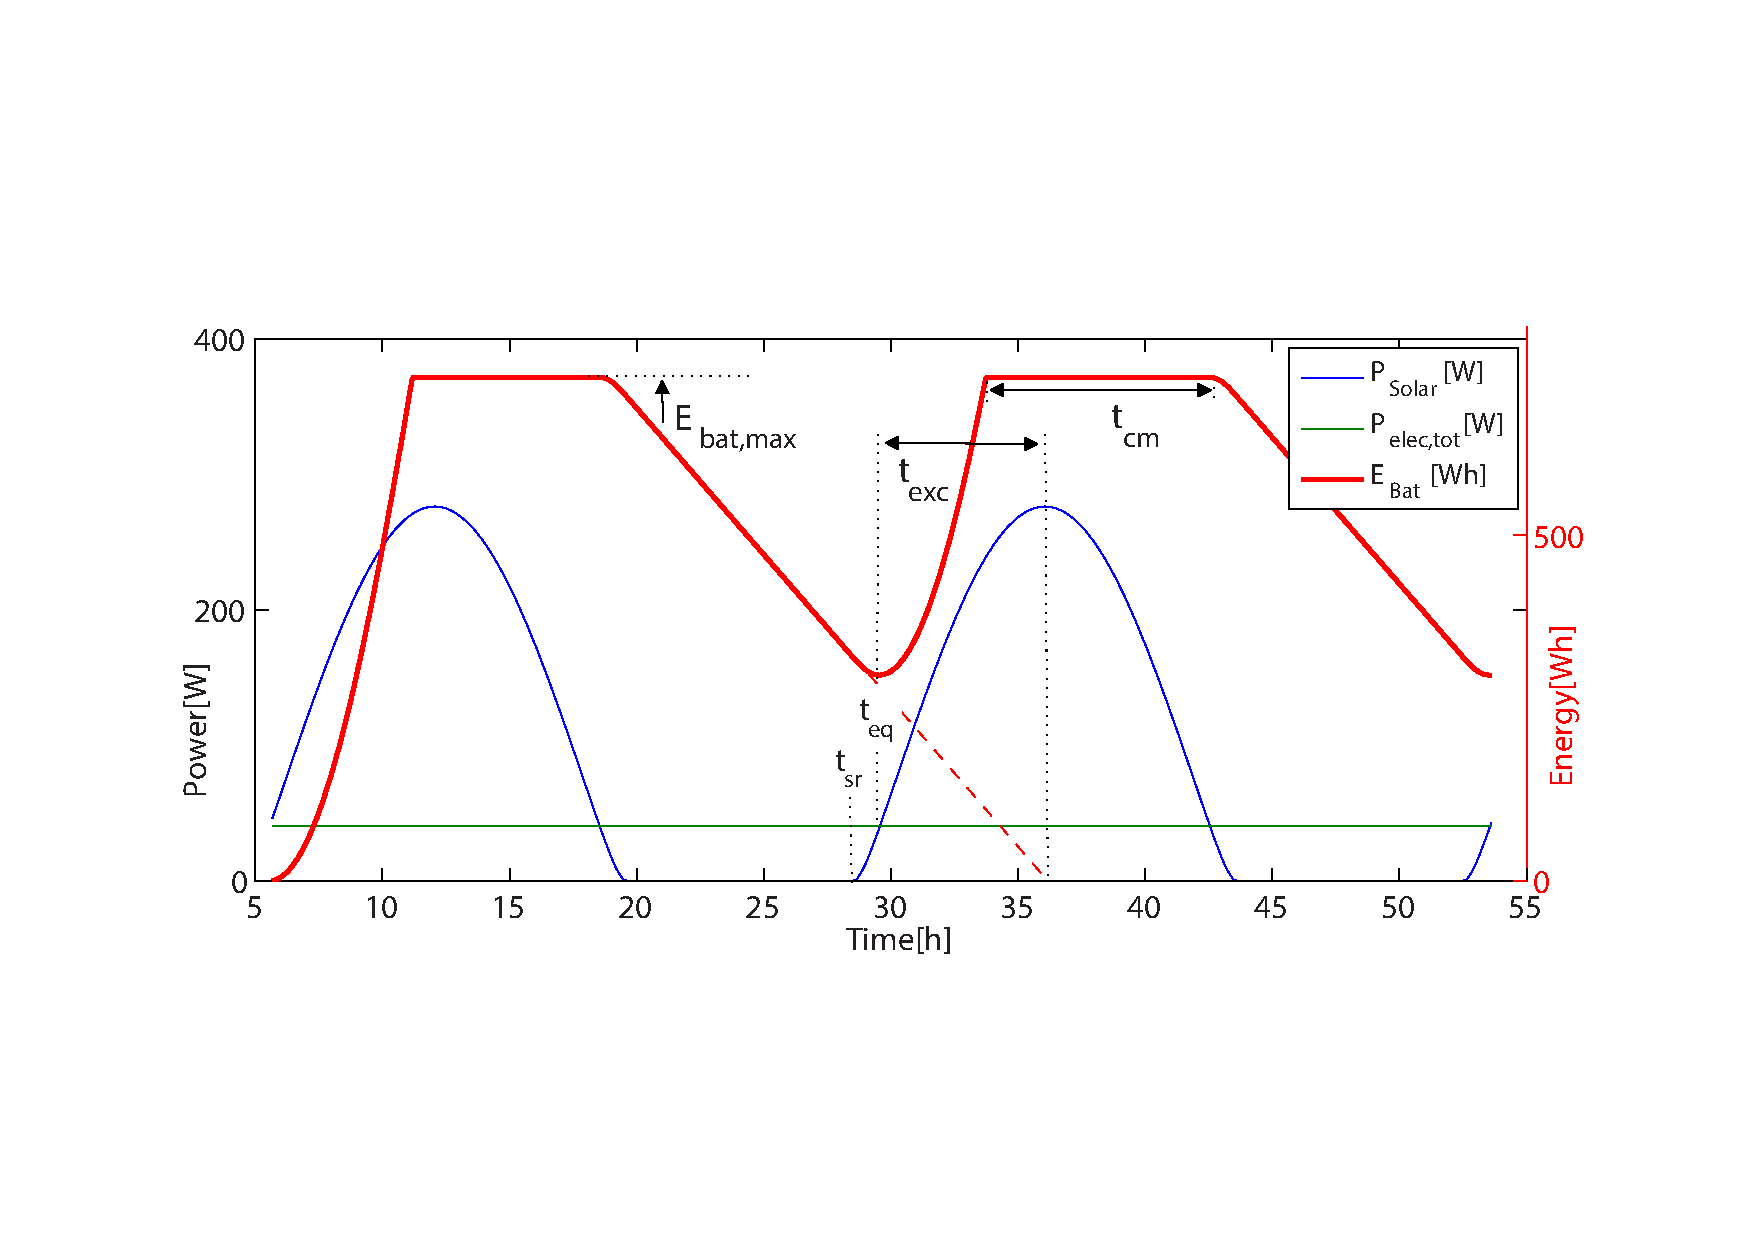
\includegraphics[width=\linewidth]{images/2_EnergySimulation.pdf}
    \caption{Exemplary energetic simulation of the \textit{AtlantikSolar} UAV configuration ($b=5.6m$, $\lambda=18.5$, $m_{bat}=3.5kg$), showing input and output power, battery capacity, and performance metrics excess time $t_{exc}$ and charge margin $t_{cm}$ during a 2-day flight.}
    \label{fig:EnergySimulation}
\end{figure}
Second, and more importantly, the optimization criteria are extended to achieve a more robust multi-day flight. In general, a necessary and sufficient condition for perpetual flight is that the excess time $t_{exc}>0$, where
\begin{equation} \label{eqn:t_exc}
t_{exc}=\frac{E_{bat}(t=t_{eq})}{P_{out}^{\,nom}} \Big| _{P_{solar}(t>t_{sr})=0}
\end{equation}
with \textit{power-equality time} $t_{eq}=t(P_{solar}^{\,nom}=P_{out}^{\,nom})$ in the morning. This means that remaining battery capacity has to exist at $t=t_{eq}$ to continue flight for instance in case of cloud coverage. Therefore, the authors in \cite{Noth_PhD,Leutenegger_JIRS} focus on maximizing $t_{exc}$. However, a large $t_{exc}$ does not provide direct robustness against disturbances in $P_{solar}$ e.g. due to cloud obstruction during the charging process. In contrast, when optimizing purely for $t_{exc}$, the methodology in Sec. \ref{sec:ConceptualDesignMethodology} will select the largest battery size (due to the scaling of $P_{level}$ with $m_{bat}$) which can be fully charged under optimal conditions, but every reduction in $P_{solar}$ will directly decrease $t_{exc}$ due to only partially charged batteries. Thus, we introduce the charge margin $t_{cm}$ as the time margin between achieving the full charge $E_{bat}=E_{bat}^{\,max}$ and restart of the discharge in the evening. In case of decreased solar power income, $t_{cm}>0$ provides additional margin before a decrease in excess time occurs.

The overall approach for increasing robustness with respect to local power disturbances is thus to determine the lowest acceptable $t_{exc}$ satisfying the UAV application requirements, and then to optimize the configuration for $t_{cm}$. The exact procedure applied is:
\vspace{-3ex}
\begin{algorithm}[htp]
  \SetAlgoLined\DontPrintSemicolon
  \SetKwFunction{proc}{}
  \SetKwProg{myproc}{}{}{}
  \myproc{} %\proc{}
  {
  \nl Choose nominal operating latitude $\varphi$, and Day of Operation $DoY^{nom}$ and the outermost days where perpetual UAV endurance is required $DoY^{\min,\max}$ \;
  \nl For the range of $DoY=[DoY^{\min},DoY^{\max}]$ obtain $t_{night}^{\min},~t_{night}^{\max}$ from~\cite{Duffie_SolarEngineering} \;
  \nl The required excess time $t_{exc,req}$ is now the sum of  \; 
  \pushline
  \nonl \scriptsize$\bullet$\normalsize~  $t_{exc,DoY} = t_{night}^{\,max}-t_{night}^{\,min}$ \;
  \nonl \scriptsize$\bullet$\normalsize~  $t_{exc,clouds}$, to allow a margin for clouds in the morning or evening \;
  \nonl \scriptsize$\bullet$\normalsize~  $t_{exc,P_{level}}$, to allow a margin for increased power consumption e.g. caused by downdrafts or uncertainties in estimating $P_{level}$ \;
  \popline \nl 
  \nl Perform the design analysis given the methodology in Section~\ref{sec:ConceptualDesignMethodology} for $DoY(t_{night}=t_{night}^{\,min})$. Pre-select the subset $\pazocal{S}$ of configurations satisfying $t_{exc}>t_{exc,req}$  \;
  \nl Within $\pazocal{S}$, allow for a set of intermediate configurations $\pazocal{S}_i$ to take into account UAV-specific constraints on $b$, $\lambda$, or $m_{bat}$. Then choose the final configuration $\pazocal{S}_f$  from $\pazocal{S}_i$ to obtain the largest charge margin $t_{cm}$ % \; 

 }
  %\caption{Inor}
\end{algorithm}

This conceptual design methodology is applied below. An alternative conceptual design approach utilizing a weighted version of $t_{exc}$ and $t_{cm}$ is proposed in \cite{Morton_ICRA2013}. 

%%%%%%%%%%%%%%%%%%%%%%%%%%%%%%%%%%%%%%%%%%%%%%%%%%%%%%%%%%%%%%%%%%%%%%%%%%%%%%%
\subsection{Application of Conceptual Design Methodology} \label{sec:ConceptDesignApplication}
%%%%%%%%%%%%%%%%%%%%%%%%%%%%%%%%%%%%%%%%%%%%%%%%%%%%%%%%%%%%%%%%%%%%%%%%%%%%%%%

\textit{AtlantikSolar} operates at a nominal latitude of $\varphi=45\degree N$ and shall provide perpetual endurance within a +/-2 month window around $DoY_{nom}$=June 21\textsuperscript{st} (April 21\textsuperscript{st}-August 21\textsuperscript{st}). From \cite{Duffie_SolarEngineering},we find $t_{night}^{\,min}=8.7h$ (June 21\textsuperscript{st}), $t_{night}^{\,max}=10.5h$(April 21\textsuperscript{st}), and thus $t_{exc,DoY}=1.80h$. We choose $t_{exc,clouds}=3.0h$ to account for three hours of full cloud coverage either on the evening or the morning and choose $t_{exc,P_{level}}=0.2\cdot t_{night,max}=2.1h$ to cover increased power consumption due to modeling errors, downdrafts or headwinds. Using $t_{exc,req}=t_{exc,DoY}+t_{exc,clouds}+t_{exc,P_{level}}$, we retrieve $t_{exc,req}=6.9h$ as the minimum required excess time for robust perpetual flight at the given dates and locations. 

The design methodology tool of Section \ref{sec:ConceptualDesignMethodology} is now applied assuming the fixed parameters in Table \ref{tab:ConceptDesignParameters}. Figure \ref{fig:ExcessTimeChargeMargin} shows the resulting plot for $t_{exc}$ versus the optimization variables $b$ and $m_{bat}$. The subset $\pazocal{S}$ of configurations satisfying $t_{exc}>t_{exc,req}$ is the region within the blue contour-line. The optimum clearly occurs at large wingspans. However, considering that we aim for a small-scale and hand-launchable configuration that allows easy transportation (in this case via disassembly of the main wing into three pieces of less than $2m$ wingspan) we choose $b=5.6m$.  The aspect ratio $\lambda=18.5$ is found to provide an optimum in $t_{exc}$ and also allows to seamlessly integrate the 125mm-wide solar cells (see Section \ref{secsec:Airframe and hardware}) inside the wing chord. The last design choice is $m_{bat}$, for which we seek to optimize $t_{cm}$ within the previously selected set $\pazocal{S}_i=(\pazocal{S}|_{b=5.6m, \lambda=18.5})$. As visible in Figure \ref{fig:ExcessTimeChargeMargin}, $m_{bat}=3.0...7.5kg$ lies within $\pazocal{S}_i$. We choose $m_{bat}=3.5kg$ to optimize $t_{cm}$ and due to practical battery sizing constraints described in Section \ref{secsec:Airframe and hardware}. The selected final configuration $\pazocal{S}_f=(\pazocal{S}|_{m_{bat}=3.5kg, b=5.6m, \lambda=18.5})$ yields an estimated $m_{tot}=7.22kg$, $t_{exc}=7.89h$ and $t_{cm}=8.38h$ for the nominal operating date and latitude.
\begin{figure}[tb]
    \centering
    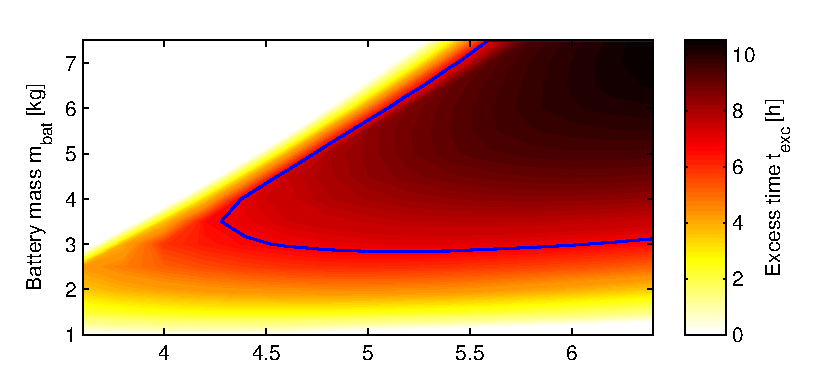
\includegraphics[width=\linewidth]{images/3_excesstime}
    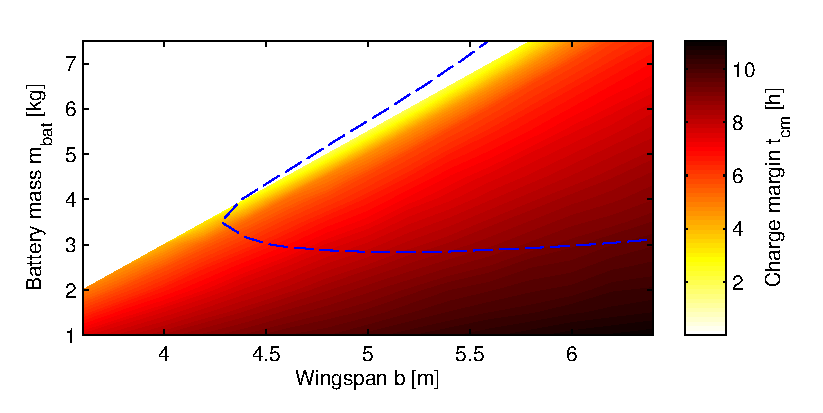
\includegraphics[width=\linewidth]{images/4_chargemargin}
    \caption{Excess time $t_{exc}$ (top) and charge margin $t_{cm}$ (bottom) vs. $b$ and $m_{bat}$, all at $\lambda=18.5$. The configuration subset $\pazocal{S}$ satisfying $t_{exc}>t_{exc,req}$ under our design requirements lies inside the blue contour line.}
    \label{fig:ExcessTimeChargeMargin}
\end{figure}
\begin{table}[h] 
\caption{Fixed parameters for the conceptual design} \label{tab:ConceptDesignParameters}
\begin{center}
\begin{tabular}{l l l}
\toprule
 Parameter & Value & Description\\ 
\midrule
 $\eta_{sm}$ & 0.20&Solar module efficiency\\
 $\eta_{MPPT}$ & 0.97&MPPT efficiency\\
 $\eta_{prop}$ & 0.58 &Propulsion system efficiency\\
 $e_{bat}$ & 874800\unitfrac{J}{kg}&Battery specific energy\\
 $f_{sm}$ & 0.94&Solar module fill factor\\
 $k_{sm}$ & 0.59$\unitfrac{kg}{m²}$ & Solar module areal density\\
 $m_{av}$ & 0.6kg&Avionics mass (including all cabling)\\
 $m_{pld}$ & 0.1kg&Payload mass\\
 $P_{av}$ & 4.5\unit{W}&Avionics power consumption\\
 $P_{pld}$ & 0.0\unit{W}&Payload power consumption\\
\bottomrule
\end{tabular}
\end{center}
\end{table}

%%%%%%%%%%%%%%%%%%%%%%%%%%%%%%%%%%%%%%%%%%%%%%%%%%%%%%%%%%%%%%%%%%%%%%%%%%%%%%%
\subsection{Robustness Analysis}
%%%%%%%%%%%%%%%%%%%%%%%%%%%%%%%%%%%%%%%%%%%%%%%%%%%%%%%%%%%%%%%%%%%%%%%%%%%%%%%

To verify the multi-day flight robustness of the developed UAV configuration, we analyze its performance considering a set of local disturbances in UAV power input and output, namely
 \begin{enumerate}[(a)]
\item The disturbed solar power income $P_{solar}^{\,dist}$, as caused by clouds or fog. Lacking knowledge of the exact spatial and temporal disturbance distribution, we assume
\begin{equation}
P_{solar}^{\,dist}(t) = P_{solar}^{\,nom}(t) \cdot k_{CCF}.
\end{equation}
Here, $k_{CCF} \in (0,1]$  represents the current cloud cover factor \cite{Kimura_SolarRadAndClouds}, i.e. the clearness of the atmosphere.
\item The disturbed electrical power output $P_{out}^{\,dist}$. Wind downdrafts, head wind, or gusts may require increased propulsion or actuation power. Again, we assume 
\begin{equation}
P_{out}^{\,dist}(t) = P_{out}^{\,nom}(t) \cdot k_{OPF},~k_{OPF} \in (0,1)
\end{equation}
with $k_{OPF}$ representing the Output Power Factor.
\end{enumerate}
\begin{figure}
    \centering
    \includegraphics[width=\linewidth]{images/5_texcRobustness/5_texcRobustness.pdf}
    %\includegraphics[width=\linewidth]{images/old/5_texcRobustness.pdf}
    \caption{Excess time under disturbed power input and output for the $b=5.6m$, $\lambda=18.5$ configuration: a) $m_{bat}$=3.5kg on June 21\textsuperscript{st} b) $m_{bat}=6.0kg$ on June 21\textsuperscript{st} c) $m_{bat}$=3.5kg on April 21\textsuperscript{st} d) $m_{bat}=6.0kg$ on April 21\textsuperscript{st} }
    \label{fig:ExcessTimeRobustness}
\end{figure}
Figure \ref{fig:ExcessTimeRobustness} shows the remaining excess time with respect to these disturbances. The UAV configuration developed in Section \ref{sec:ConceptDesignApplication} ($m_{bat}=3.5kg$) still provides perpetual endurance with less than 50\% of the solar power income or if more than 60\% increased power are required on June 21\textsuperscript{st} (Figure \ref{fig:ExcessTimeRobustness}a). In contrast, a configuration purely optimized towards excess time ($m_{bat}=6.0kg$, Figure \ref{fig:ExcessTimeRobustness}b) will yield a higher maximum $t_{exc}$ of 9.5h, but the robustness with respect to clouds or higher required level power is greatly decreased. On April  21\textsuperscript{st}, the UAV configuration of Section \ref{sec:ConceptDesignApplication} still provides solid robustness (Figure \ref{fig:ExcessTimeRobustness}c), which verifies the $DoY^{\,nom}\pm$ 2 months perpetual endurance requirement. In contrast, the $m_{bat}=6.0kg$ configuration (Figure \ref{fig:ExcessTimeRobustness}d) can not provide reliable perpetual endurance anymore. Overall, the configuration developed using the extended optimization criteria from Section \ref{sec:ExtensionOptCriteria} thus shows significantly improved multi-day flight robustness in comparison with configurations that are purely optimized for maximum excess time.

%%%%%%%%%%%%%%%%%%%%%%%%%%%%%%%%%%%%%%%%%%%%%%%%%%%%%%%%%%%%%%%%%%%%%%%%%%%%%%%
% SECTION3: DETAILED DESIGN AND REALIZATION
%%%%%%%%%%%%%%%%%%%%%%%%%%%%%%%%%%%%%%%%%%%%%%%%%%%%%%%%%%%%%%%%%%%%%%%%%%%%%%%
%%%%%%%%%%%%%%%%%%%%%%%%%%%%%%%%%%%%%%%%%%%%%%%%%%%%%%%%%%%%%%%%%%%%%%%%%%%%%%%
\section{DETAILED DESIGN AND REALIZATION}
%%%%%%%%%%%%%%%%%%%%%%%%%%%%%%%%%%%%%%%%%%%%%%%%%%%%%%%%%%%%%%%%%%%%%%%%%%%%%%%

AtlantikSolar (Fig. \ref{fig:AtlantikSolarCollage}) is a solar-powered Low-Altitude Long-Endurance(LALE) UAV designed and built at ETH Zurich for perpetual flight at $\varphi=45°$ geographical latitude from April 21\textsuperscript{st} to August 21\textsuperscript{st}. Although its design is mostly dictated by the requirement for low level-flight power consumption, it provides means to mount an advanced optical\&infrared sensor pod developed at ETH Zurich for use in autonomous search and rescue or industrial inspection missions. The airplane airframe characteristics are summarized in table \ref{tab:DetailedDesignParameters}. An overview over the airplane system topology is given in Fig. \ref{fig:AtlantikSolar_SystemOverview}.

\begin{figure}[h]
    \centering
    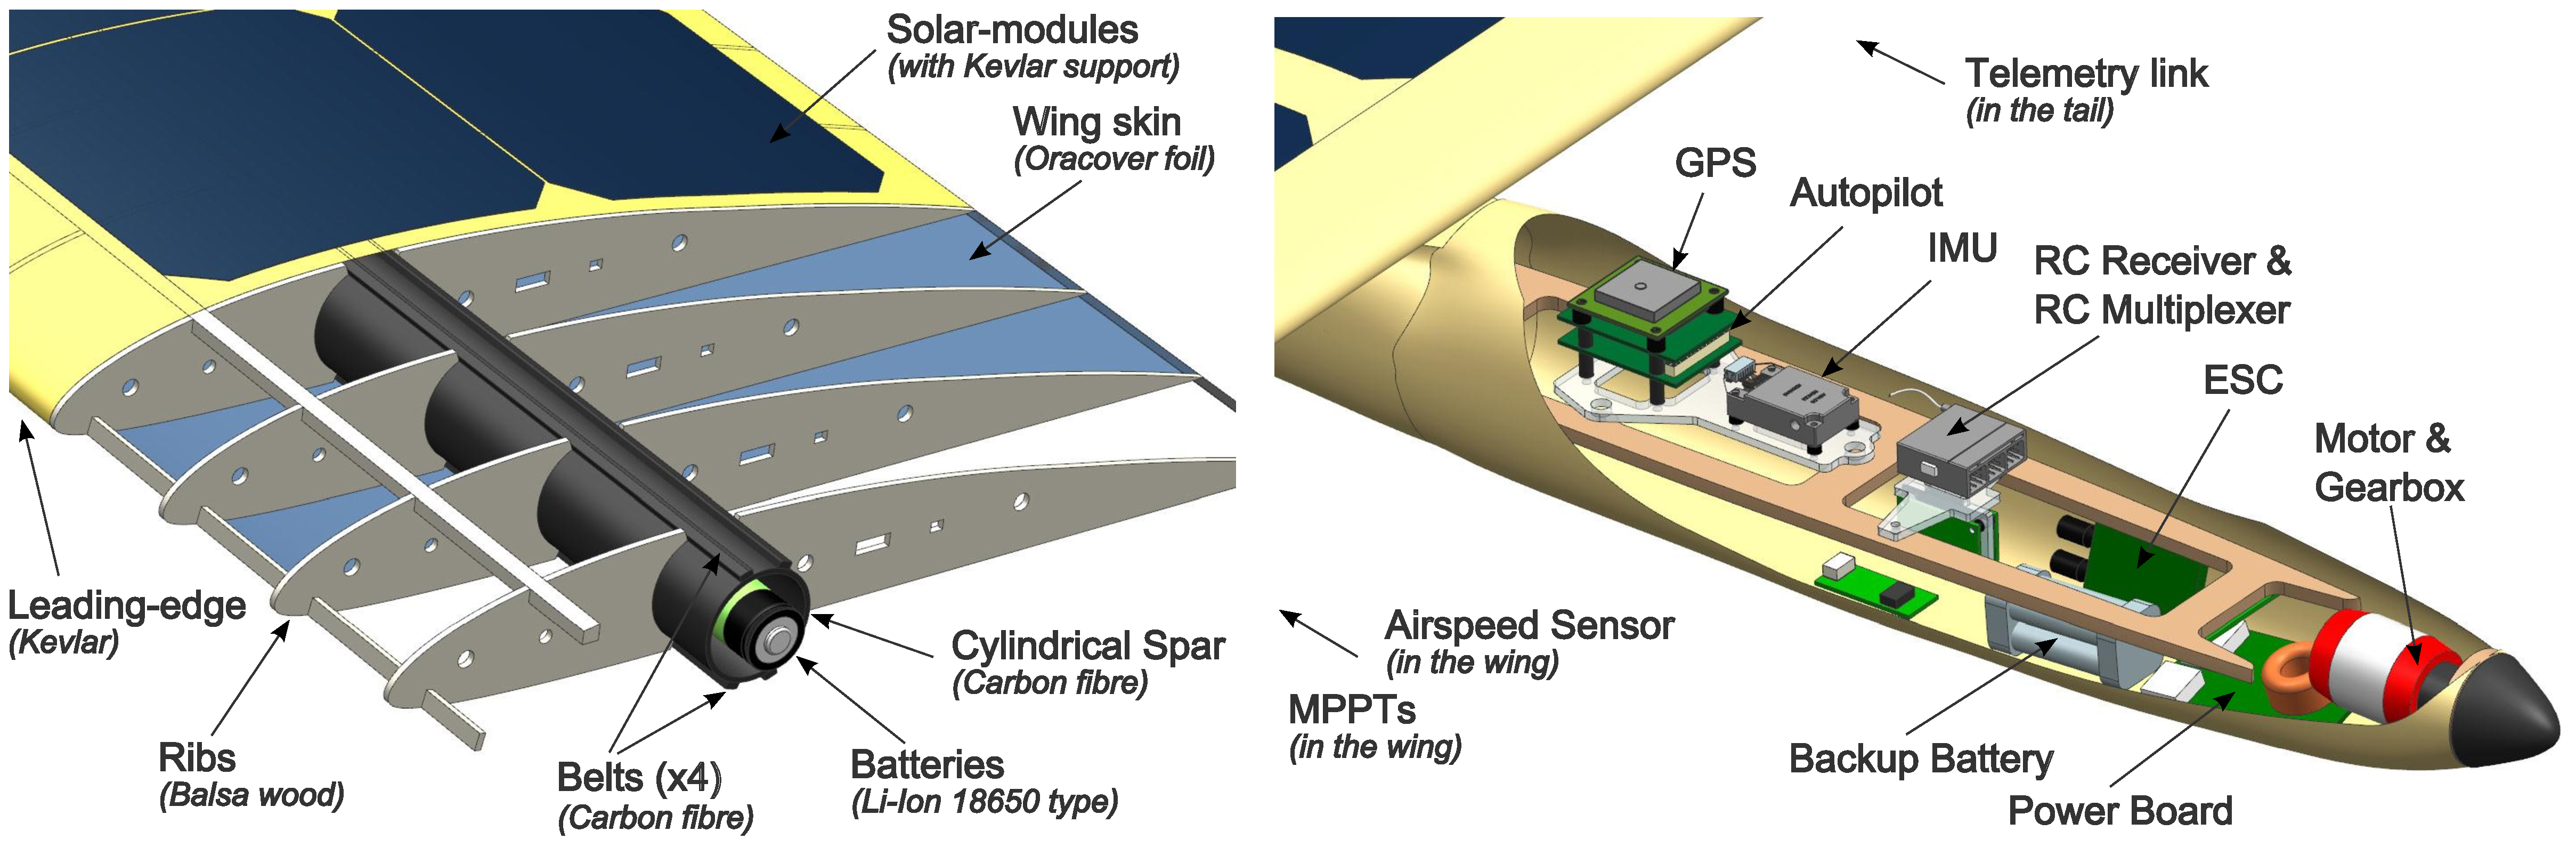
\includegraphics[width=\linewidth]{images/10_CAD_AtlantikSolarAvionics_Combined}
    \caption{Left: Wing structure with integrated batteries and solar cells. Right: Main avionics layout inside the airplane.}
    \label{fig:CAD_AtlantikSolarStructureAndAvionics}
\end{figure}
%\begin{figure}[tb]
%    \centering
%    \includegraphics[width=\linewidth]{images/6_CAD_AtlantikSolarFull}
%    \caption{The AtlantikSolar UAV features a conventional T-tail configuration with 1 motor, two ailerons, an all-moving elevator and a rudder for actuation.}
%    \label{fig:CAD_AtlantikSolarFull}
%\end{figure}

\begin{table}
\caption{AtlantikSolar design characteristics}
\label{tab:DetailedDesignParameters}
\begin{center}
\begin{tabular}{l l}
Wing span & 5.65$\unit{m}$\\
\hline Wing chord& 0.305$\unit{m}$\\
\hline Length& 2.03\unit{m}\\
\hline Height&0.45\unit{m}\\
\hline Mass& 7.36$\unit{kg}$\\
\hline Battery mass& 3.52$\unit{kg}$\\
\hline Wing loading&4.28$\unitfrac{kg}{m^2}$\\
\hline Stall speed& 8.1$\unitfrac{m}{s}$\\
\end{tabular}
\end{center}
\end{table}

%%%%%%%%%%%%%%%%%%%%%%%%%%%%%%%%%%%%%%%%%%%%%%%%%%%%%%%%%%%%%%%%%%%%%%%%%%%%%%%
\subsection{UAV Platform Design}
%%%%%%%%%%%%%%%%%%%%%%%%%%%%%%%%%%%%%%%%%%%%%%%%%%%%%%%%%%%%%%%%%%%%%%%%%%%%%%%

%%%%%%%%%%%%%%%%%%%%%%%%%%%%%%%%%%%%%%%
\subsubsection{Airframe}\label{secsec:Airframe and hardware}
%%%%%%%%%%%%%%%%%%%%%%%%%%%%%%%%%%%%%%%
The structure of AtlantikSolar is built in a traditional rib-spar construction method (Fig. \ref{fig:CAD_AtlantikSolarStructureAndAvionics}). The wing's main element is an inner cylindrical carbon-fibre spar to resist torsional wing loads. Four carbon-fibre belts of trapezoidal and laterally-varying cross-section are attached to the spar to optimally resist bending loads and to provide maximum wing stiffness to structurally unload the wing surface and especially the solar cells. The main wing can be disassembled into three wing pieces of $b<2m$ each. The horizontal and vertical stabilizers are built as the main wing.

%%%%%%%%%%%%%%%%%%%%%%%%%%%%%%%%%%%%%%%
\subsubsection{Energy Generation and Storage}
%%%%%%%%%%%%%%%%%%%%%%%%%%%%%%%%%%%%%%%
The cylindrical wing spars are fitted with 72 cylindrical high energy-density industrial Lithium-Ion battery cells (Panasonic NCR18650b, 243Wh/kg) to optimally distribute the battery mass in a ``span loader'' concept. The cells are connected in a 6S (22.2V) configuration and provide $E_{bat,max}=850Wh$ at $m_{bat}=3.5kg$. The solar modules feature a total of 88 SunPower C60 cells with a measured module-level efficiency of $\eta_{sm}=0.20$, an areal density of $k_{sm}=590g/m^2$ and a maximum power output of 275W at $\varphi=45°$ on June 21\textsuperscript{st}. Modules featuring SunPower E60 cells with a measured \cite{Sunier_EPFLSolarModules} $\eta_{sm}=0.23$ are currently being integrated. The solar modules are seamlessly embedded in the upper wing surface to avoid premature flow separation.

\begin{figure}[tb]
    \centering
     \includegraphics[width=\linewidth]{images/8_AtlantikSolar_Avionics}
    \caption{AtlantikSolar system overview. For clarity, voltage lines from the autopilot to connected devices (5.0V and 3.3V) are omitted.}
    \label{fig:AtlantikSolar_SystemOverview}
\end{figure}

%%%%%%%%%%%%%%%%%%%%%%%%%%%%%%%%%%%%%%%
\subsubsection{Actuation}
%%%%%%%%%%%%%%%%%%%%%%%%%%%%%%%%%%%%%%%
The propulsion system features a foldable custom built carbon-fibre propeller with diameter $D=66cm$ and pitch $H=60cm$. It is driven by a 5:1 reduction-ratio planetary gearbox, a RS-E Strecker 260.20 brushless DC motor with $k_V=570RPM/V$ and a Kontronik Koby 55 LV motor controller at up to $P_{prop,max}=450W$ electrical input power. The actuation system consists of four Volz DA-15N servos that drive the two ailerons, the all-moving elevator and the rudder. To guarantee reliable multi-day flight, the Volz actuators were successfully bench-tested throughout a simulated continuous 30-day flight \cite{DellaCa_BT}.
%mention wind tunnel, lab motor test stand tests? Only if space left...

%%%%%%%%%%%%%%%%%%%%%%%%%%%%%%%%%%%%%%%
\subsubsection{Avionics}
%%%%%%%%%%%%%%%%%%%%%%%%%%%%%%%%%%%%%%%
The avionics installation (Figs. \ref{fig:AtlantikSolar_SystemOverview} and \ref{fig:CAD_AtlantikSolarStructureAndAvionics}) is centered around a Pixhawk PX4 Autopilot - an open source and open hardware project initiated at ETH Zurich - with a Cortex M4F microprocessor running at 168Mhz and featuring 192kB RAM. For attitude estimation (Sec. \ref{secsec:StateEstimation}), an ADIS 16448 10-axis Inertial Measurement Unit (IMU), a u-Blox LEA-6H GPS receiver, and a Sensirion SDP600 differential pressure sensor are used. The SDP600 airspeed sensor exhibits less than 5\% error at airspeeds of 8m/s, which is essential to closely control the airspeed to the minimum required power $P_{out}$ state. Both a 433Mhz medium-range telemetry link and a long-range IRIDIUM-based satellite backup link are integrated. The airplane implements a fully manual RC-command fall-back mode in case of a severe autopilot failure. Night operations are possible due to four on-board high-power indicator LEDs.

%\begin{figure}[tb]
%    \centering
%    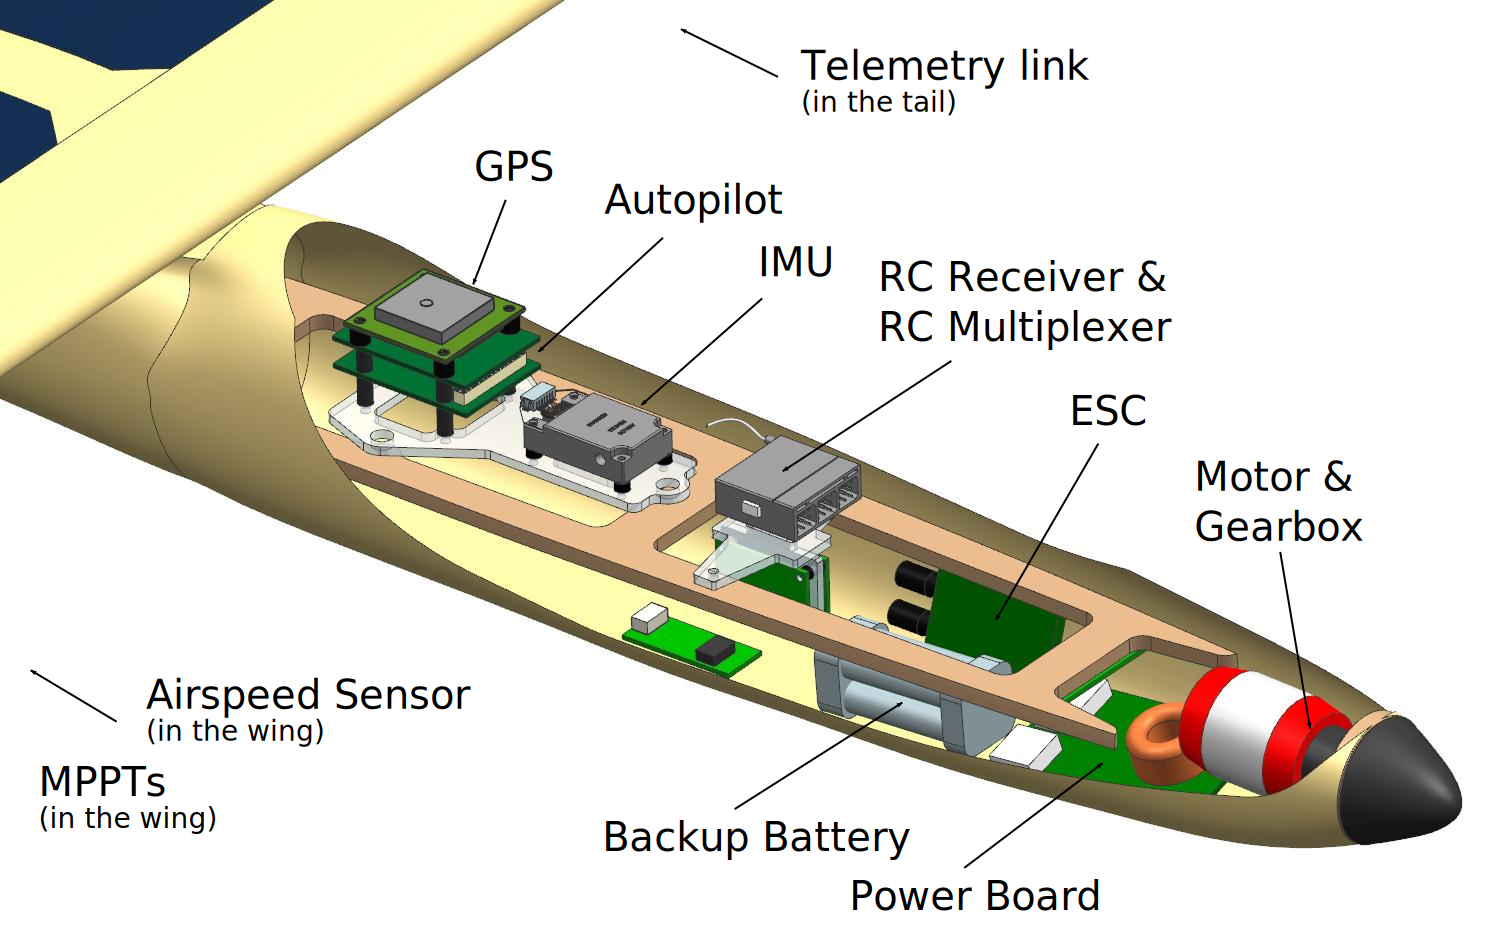
\includegraphics[width=\linewidth]{images/9_CAD_AtlantikSolarAvionics}
%    \caption{Avionics components and their placement inside AtlantikSolar.}
%    \label{fig:9_CAD_AtlantikSolarAvionics}
%\end{figure}

%%%%%%%%%%%%%%%%%%%%%%%%%%%%%%%%%%%%%%%
\subsubsection{Payload}
%%%%%%%%%%%%%%%%%%%%%%%%%%%%%%%%%%%%%%%
% [THOMAS]
  - VI Sensor [ref to VI-sensor paper; ref to Leutenegger thesis?]
  - ~5 sentences + 1 picture
  
%%%%%%%%%%%%%%%%%%%%%%%%%%%%%%%%%%%%%%%%%%%%%%%%%%%%%%%%%%%%%%%%%%%%%%%%%%%%%%%
\subsection{State Estimation and Control Design}
%%%%%%%%%%%%%%%%%%%%%%%%%%%%%%%%%%%%%%%%%%%%%%%%%%%%%%%%%%%%%%%%%%%%%%%%%%%%%%%

%%%%%%%%%%%%%%%%%%%%%%%%%%%%%%%%%%%%%%%
\subsubsection{State Estimation} \label{secsec:StateEstimation}
%%%%%%%%%%%%%%%%%%%%%%%%%%%%%%%%%%%%%%%
% [AMIR]
  - brief (5 sentence) description of SE type/principle
  - one verification plot (e.g. gps position ``ground truth'' vs. estimated position) 
  then REF to stefan\&Amir paper
  
%%%%%%%%%%%%%%%%%%%%%%%%%%%%%%%%%%%%%%%
\subsubsection{System Identification} \label{sec:SystemID}
%%%%%%%%%%%%%%%%%%%%%%%%%%%%%%%%%%%%%%%
%[DR. ALEXIS]
 - System Identification \& Modelling
 
 %	This subsection overviews the system identification methods employed for AtlantikSolar

Towards aiding the control synthesis procedure, a simplified linear state--space representation of the UAV dynamics was also derived based on recorded flight data and frequency--domain system identification methods. For non--aggressive maneuvering and around level flight, linear models may capture the vehicle response for small perturbations around a given equilibrium. Decoupling the longitudinal and lateral axis the dynamics of a UAV may take the following form~\cite{dorobantu2011frequency,OMLAS_MED_2014}: 

\small
\begin{eqnarray}\label{LON_DYN}
 \mathbf{M}_{lon}\dot{\mathbf{x}}_{lon} &=& \mathbf{A}^\prime_{lon}\mathbf{x}_{lon}+\mathbf{B}^\prime_{lon}u_{elev} \\ \nonumber
 \mathbf{x}_{lon} &=& \left[ u~w~q~\theta \right]^T
\end{eqnarray}
\normalsize
where $u,w,q,\theta$ correspond to the body $x$--axis, $z$--axis velocities, the pitch rate and the pitch angle respectively, $u_{elev}$ corresponds to the elevator deflection and

\scriptsize
\begin{eqnarray}
\mathbf{M}_{lon} &=& \begin{bmatrix}
m & 0 & 0 & 0\\ 
0 & m & 0 & 0\\ 
0 & 0 & I_y & 0\\ 
0 & 0 & 0 & 1
\end{bmatrix},\\ \nonumber
\mathbf{A}^\prime_{lon} &=& \begin{bmatrix}
X_u & X_w & X_q-mW_e & -mg\cos\theta_e\\ 
Z_u & Z_w & Z_q+mU_e & -mg\sin\theta_e\\ 
M_u & M_w & M_q & 0 \\ 
0 & 0 & 1 & 0
\end{bmatrix}~
\mathbf{B}^\prime_{lon} = \begin{bmatrix}
X_{u_{elev}}\\ 
Z_{u_{elev}}\\ 
M_{u_{elev}}\\ 
0
\end{bmatrix}
\end{eqnarray}
\normalsize
where $m$ is the mass, $I_y$ the inertia around the body $y$--axis, $W_e,\theta_e$ are the trimming points of vertical velocity and pitch angle, and the elements of $\mathbf{M}_{lon},\mathbf{A}^\prime_{lon}$ and $\mathbf{B}^\prime_{lon}$ form the stability and control derivatives of the UAV longitudinal dynamics. 

Similarly, for the lateral dynamics the model takes the following form:


\small
\begin{eqnarray}\label{LAT_DYN}
 \mathbf{M}_{lat}\dot{\mathbf{x}}_{lat} &=& \mathbf{A}^\prime_{lat}\mathbf{x}_{lat}+\mathbf{B}^\prime_{lat}u_{elev} \\ \nonumber
 \mathbf{x}_{lat} &=& \left[v~p~r~\phi \right]^T
\end{eqnarray}
\normalsize
where $v,p,r,\phi$ correspond to the body $y$--axis velocity, the roll and yaw rates and roll angle respectively, $u_{ail}$ is the aileron deflection, $u_{rud}$ is the rudder deflection and

\scriptsize
\begin{eqnarray}
\mathbf{M}_{lat} &=& \begin{bmatrix}
m & 0 & 0 & 0\\ 
0 & I_x & -I_{xz} & 0\\ 
0 & -I_{xz} & I_z & 0\\ 
0 & 0 & 0 & 1
\end{bmatrix},\\ \nonumber 
\mathbf{A}^\prime_{lat} &=& \begin{bmatrix}
Y_v & Y_p + mW_e & Y_r-mU_e & mg\cos\theta_e\\ 
L_v & L_p & L_r & 0\\ 
N_v & N_p & N_r & 0 \\ 
0 & 1 & \tan\theta_e & 0
\end{bmatrix},~ \mathbf{B}^\prime_{lat} = \begin{bmatrix}
Y_{u_{ail}} & Y_{u_{rud}}\\ 
L_{u_{ail}} & L_{u_{rud}}\\ 
N_{u_{ail}} & N_{u_{rud}}\\ 
0 & 0
\end{bmatrix}
\end{eqnarray}
\normalsize
where $I_x$ the inertia around the body $x$--axis, $I_{xz}$ the cross--inertia term of the body $x,z$--axes and the elements of $\mathbf{M}_{lat},\mathbf{A}^\prime_{lat}$ and $\mathbf{B}^\prime_{lat}$ form the stability and control derivatives of the UAV lateral dynamics. 
 
 %%%%%%%%%%%%%%%%%%%%%%%%%%%%%%%%%%%%%%%
 \subsubsection{Control}
 %%%%%%%%%%%%%%%%%%%%%%%%%%%%%%%%%%%%%%%
 %[PHILIPP writes this, DR. ALEXIS checks this]

%	This subsection provides some info on the controllers that run on AtlantikSolar

\begin{figure}[tb]
    \centering
     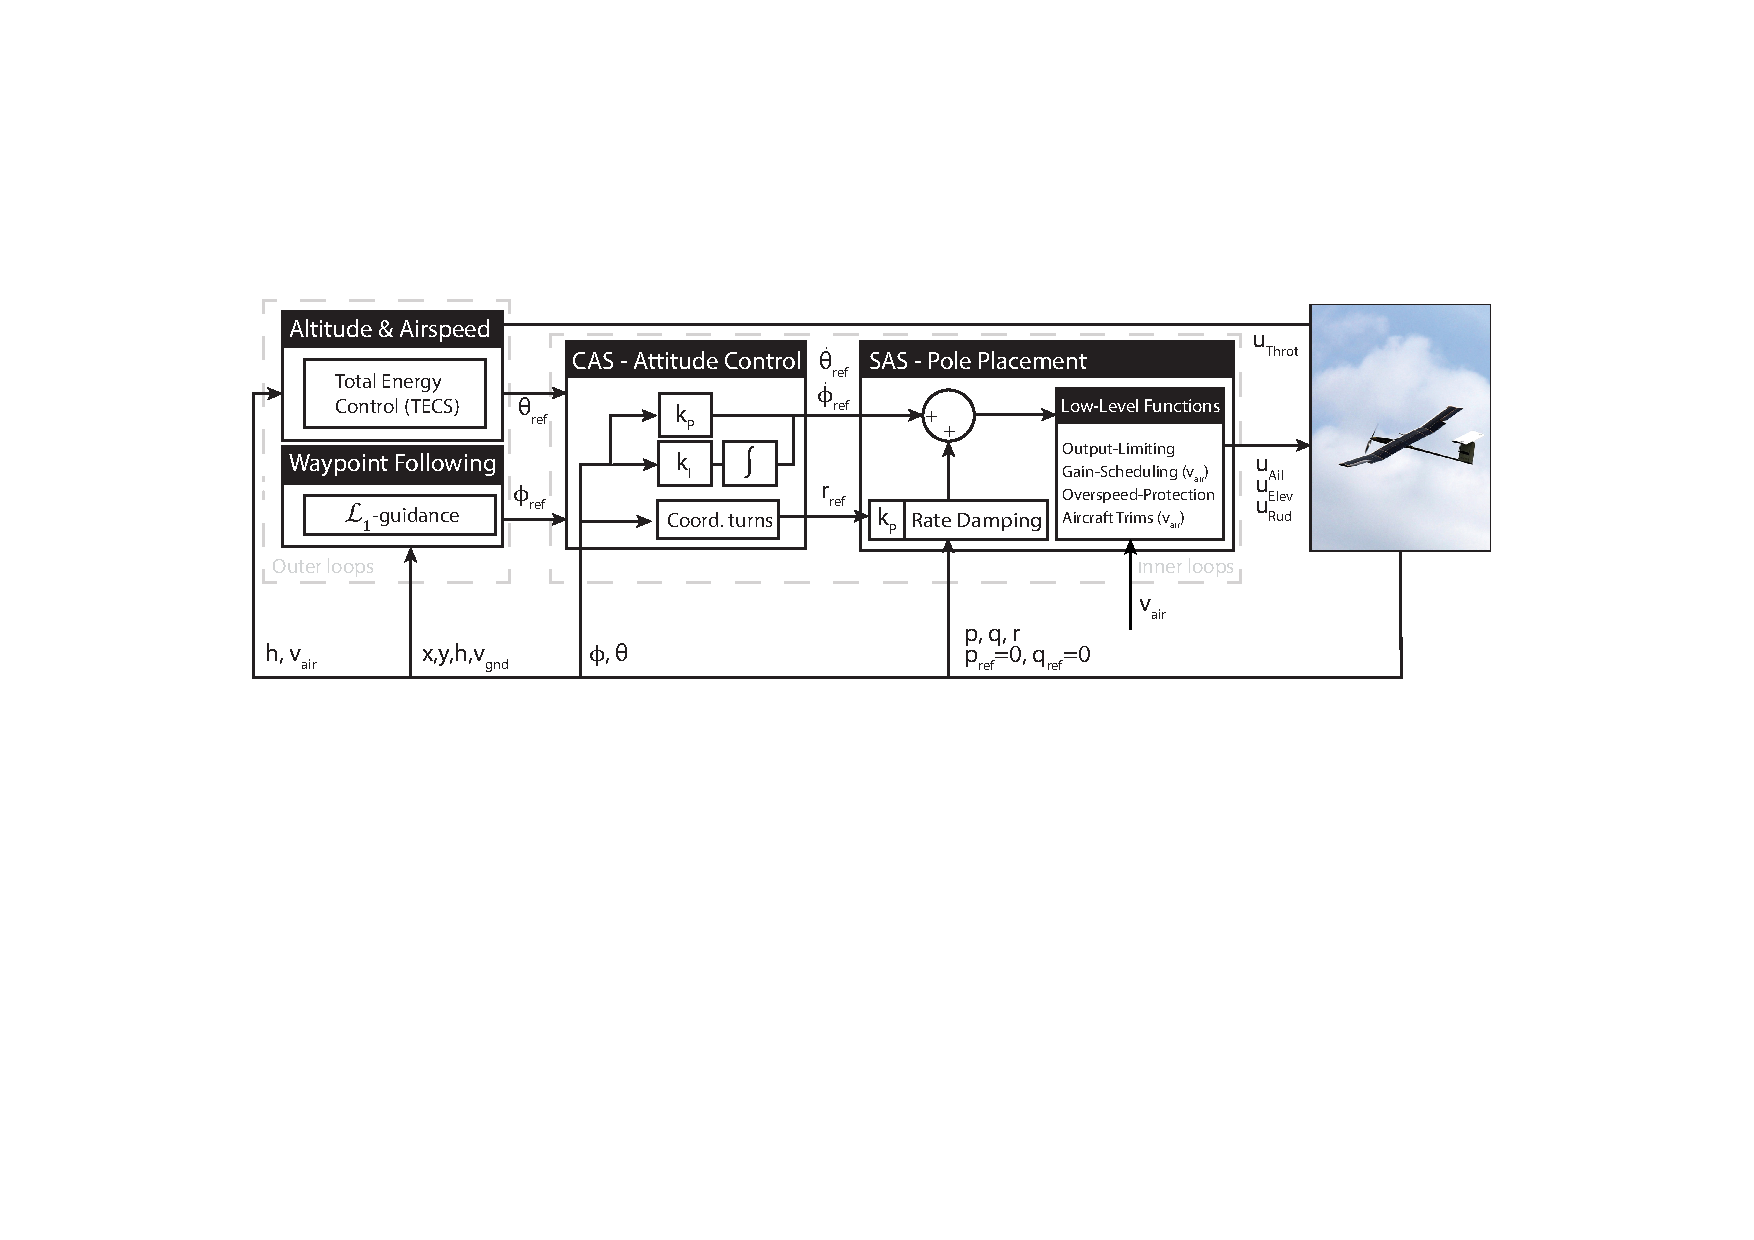
\includegraphics[width=\linewidth]{images/11_ControlScheme/ControlScheme.pdf}
    \caption{Control Scheme implemented for AtlantikSolar.}
    \label{fig:ControlScheme}
\end{figure}

AtlantikSolar features autonomous navigation and loitering through user--defined waypoints. The complete control structure (Fig.~\ref{fig:ControlScheme}) is offline-tuned based on the identified system model (Sec.~\ref{sec:SystemID}), functionality-tested in an X--Plane 10 Hardware--In--the--Loop (HIL) simulation and finally refined in extensive flight tests. For inner--loop control, our baseline--solution corresponds to a set of cascaded saturated PID controllers: The Stability Augmentation System (SAS) applies rate--damping to shape the airplane's frequency response, while the Control Augmentation System (CAS) applies proportional--integral feedback to achieve roll ($\phi$) and pitch ($\theta$) reference tracking. As a cascaded approach, proper tuning requires iteration of the gains to achieve maximum performance and robustness against model uncertainties and external disturbances. Flight tests showed that due to AtlantikSolar's high wingspan and thus high x- and z-axis inertia $I_x$ and $I_z$, coordinated turn control is essential to damp adverse yaw and to achieve the no--sidelslip yaw rate $r=\frac{g\cdot \sin(\phi)}{v_{air}}$. To avoid overload of the highly optimized structure, output limiters and an over--speed protection are applied. Furthermore, the control actions are in a final stage adapted with respect to the dynamic pressure $q=\frac{1}{2}\rho v^{2}_{air}$ which accounts for the change of the effective moments created by the control surfaces. 

Once the inner--loops are well--tuned, waypoint guidance is enabled. AtlantikSolar employs a $\mathcal{L}_1$--nonlinear guidance law which generates the lateral acceleration reference $a_{s_{ref}}$ of the UAV based on a look--ahead distance ${L}_1$ and the current velocity $V_T$ and heading error $\eta$ as noted below:

\small
\begin{eqnarray}
 a_{s_{ref}} &=& 2\frac{V_T^2}{L_1}\sin \eta
\end{eqnarray}
\normalsize
which is then kinematically translated to roll references while consistent dynamic behaviour is achieved via adaptation of the look--ahead distance as in~\cite{L1stabAnalysis}. This guidance law is integrated into our control structure as described in~\cite{OMLAS_MED_14} and combined with an extended version of the Pixhawk open--source Total Enery Control System (TECS)~\cite{PixhawkWebsite} which provides altitude control: First, a slew rate constraint on the reference altitude $h_{ref}$ has been integrated to reach smoother altitude control at pre-definable climb and sink rates, which is especially important for low propulsion-power to weight-ratio UAVs such as AtlantikSolar. Second, we have implemented \textit{thermal compliance}: In an updraft, the standard TECS implementation will decrease $\theta_{ref}$ to decrease the altitude if $h>h_{ref}$. To allow gaining potential energy from a thermal, we perform gain-scheduling on TECS configuration parameters such that $\theta_{ref}$ is used only for airspeed control and $u_{Throt}$ only for altitude control. When at $h>h_{ref}$, the plane will thus keep $\theta_{ref}=\theta_{ref}(t)$  such that $v(t)=v_{ref}(t)$ and will gradually disable the motor, potentially gaining altitude for strong thermals. Furthermore, altitude limits have been implemented, i.e. full throttle is forced for $h<h_{min}$, at $h>h_{max}$ we gradually allow a pitch-down and thus altitude decrease again, and at $h>h_{max}+50m$ the controller automatically engages the spoilers for maximum descend rate. The inner PID-based pitch- and roll control loops are executed at a sampling period of $T_{SAS,CAS}=0.01s$, while the high-level $\mathcal{L}_1$\&TECS controllers run with $T_{\mathcal{L}_1,TECS}=0.05s$. Given these settings, the full controller requires less than 4\% CPU load, 5KB of RAM and 47KB Flash memory and is thus computationally lightweight when compared to other Pixhawk applications (see~\cite{OMLAS_MED_14}) such as the state estimation. The whole control application is designed to be modular, and more sophisticated approaches like model-predictive control~\cite{OMLAS_MED_14} and robust $H_\infty$--based controllers~\cite{Mosimann_FT} for inner loop control have been implemented and flown on test planes in addition to our cascaded PID baseline-solution. 

% Verification plots:
% - Test at what winds and what performance (e.g. during loitering for power measurements -> very good tracking)
% - Later: show waypoint tracking (not loitering!) with altitude change for control (\&State Estimator) operation verification. Alternatively: Show this in the ICARUS test paths ...
% - show spoiler operation and thermal compliance operation?


%%%%%%%%%%%%%%%%%%%%%%%%%%%%%%%%%%%%%%%%%%%%%%%%%%%%%%%%%%%%%%%%%%%%%%%%%%%%%%%
% SECTION4: EXPERIMENTAL RESULTS
%%%%%%%%%%%%%%%%%%%%%%%%%%%%%%%%%%%%%%%%%%%%%%%%%%%%%%%%%%%%%%%%%%%%%%%%%%%%%%%
%%%%%%%%%%%%%%%%%%%%%%%%%%%%%%%%%%%%%%%%%%%%%%%%%%%%%%%%%%%%%%%%%%%%%%%%%%%%%%%
\section{EXPERIMENTAL RESULTS}
%%%%%%%%%%%%%%%%%%%%%%%%%%%%%%%%%%%%%%%%%%%%%%%%%%%%%%%%%%%%%%%%%%%%%%%%%%%%%%%
   
%PHILIPP]
 - mention total flight hours, total flights. Mention that 2 AtlantikSolars have already been built \& flown.  Range of weather conditions?
 
%%%%%%%%%%%%%%%%%%%%%%%%%%%%%%%%%%%%%%%%%%%%%%%%%%%%%%%%%%%%%%%%%%%%%%%%%%%%%%%
\subsection{Subsystem level results}
%%%%%%%%%%%%%%%%%%%%%%%%%%%%%%%%%%%%%%%%%%%%%%%%%%%%%%%%%%%%%%%%%%%%%%%%%%%%%%%
 
%[PHILIPP]. If not already done in the sections before.
   - power efficiency curves. P\_level from Test flights. Comparison to conceptual design. Describe why power consumption not optimal: e.g. because optimal CD/CL\^1.5 assumed, but this has a) to be met in average and b) even then fluctuations as seen in flight tests are on the order of 2-3 degrees in AOA or +/- 1m/s, so this will never be met perfectly.
 - solar system operation and recharge of batteries
 - state estimation (if not shown before)
 - control (if not shown before):   - SE\&Control: PID performance over various trim points. PID computational requirements (low!)
  
%%%%%%%%%%%%%%%%%%%%%%%%%%%%%%%%%%%%%%%%%%%%%%%%%%%%%%%%%%%%%%%%%%%%%%%%%%%%%%%
\subsection{Continuous 12hour Flight}
%%%%%%%%%%%%%%%%%%%%%%%%%%%%%%%%%%%%%%%%%%%%%%%%%%%%%%%%%%%%%%%%%%%%%%%%%%%%%%%
  
%[PHILIPP]
   - focus on battery performance. Say that even more possible (mention some results from the lab tests)
   - explain how much autonomous, under which conditions.
  
%%%%%%%%%%%%%%%%%%%%%%%%%%%%%%%%%%%%%%%%%%%%%%%%%%%%%%%%%%%%%%%%%%%%%%%%%%%%%%%
\subsection{Mapping Flights in Search and Rescue scenarios}
%%%%%%%%%%%%%%%%%%%%%%%%%%%%%%%%%%%%%%%%%%%%%%%%%%%%%%%%%%%%%%%%%%%%%%%%%%%%%%%
   
%[DRALEXIS]
    - mapping missions in ICARUS. 
    - REF to Separate paper??? Yes, but only once both are accepted.
    - some cool pics/reconstructed maps

%%%%%%%%%%%%%%%%%%%%%%%%%%%%%%%%%%%%%%%%%%%%%%%%%%%%%%%%%%%%%%%%%%%%%%%%%%%%%%%
\section{CONCLUSIONS}
 %%%%%%%%%%%%%%%%%%%%%%%%%%%%%%%%%%%%%%%%%%%%%%%%%%%%%%%%%%%%%%%%%%%%%%%%%%%%%%%
Mention:
  - Main lessons learned / summarize main points of paper
 - Future work
 
 %TODOs:
 % - table references point at section, not at table number itself!
 
%CHECK AT END:
% - all references (especially: urls, capitalization)
% - Check all equations


\addtolength{\textheight}{-12cm}   % This command serves to balance the column lengths
                                  % on the last page of the document manually. It shortens
                                  % the textheight of the last page by a suitable amount.
                                  % This command does not take effect until the next page
                                  % so it should come on the page before the last. Make
                                  % sure that you do not shorten the textheight too much.

%%%%%%%%%%%%%%%%%%%%%%%%%%%%%%%%%%%%%%%%%%%%%%%%%%%%%%%%%%%%%%%%%%%%%%%%%%%%%%%%



%%%%%%%%%%%%%%%%%%%%%%%%%%%%%%%%%%%%%%%%%%%%%%%%%%%%%%%%%%%%%%%%%%%%%%%%%%%%%%%%



%%%%%%%%%%%%%%%%%%%%%%%%%%%%%%%%%%%%%%%%%%%%%%%%%%%%%%%%%%%%%%%%%%%%%%%%%%%%%%%%
\section*{APPENDIX}

Appendixes should appear before the acknowledgment.

\section*{ACKNOWLEDGMENT}

The preferred spelling of the word �acknowledgment� in America is without an �e� after the �g�. Avoid the stilted expression, �One of us (R. B. G.) thanks . . .�  Instead, try �R. B. G. thanks�. Put sponsor acknowledgments in the unnumbered footnote on the first page.

%%%%%%%%%%%%%%%%%%%%%%%%%%%%%%%%%%%%%%%%%%%%%%%%%%%%%%%%%%%%%%%%%%%%%%%%%%%%%%%%

\bibliographystyle{IEEEtran}
\bibliography{refs/refs_SolarUAVs,refs/refs_PhilippOePapers,refs/refs_AllOthers}

\end{document}
